\vspace{1.5cm}

En la figura~\figref{fig:fig_p21}, se muestra el circuito de la fuente de alimentación basado en el \textit{LM723} que armamos usando el mismo driver de corriente que la fuente original y ajustando los resistores de tal forma de que las características de tensión, limitación de corriente, etc, se parezcan lo mas posible al circuito original, los valores de compensación se toman de circuitos recomendados.\\
Con ese circuito, adecuadamente modificado, se repitieron algunas de las simulaciones para realizar la comparación pedida.\\

\vfill


\clearpage

\begin{figure}[H] %htb
\begin{center}
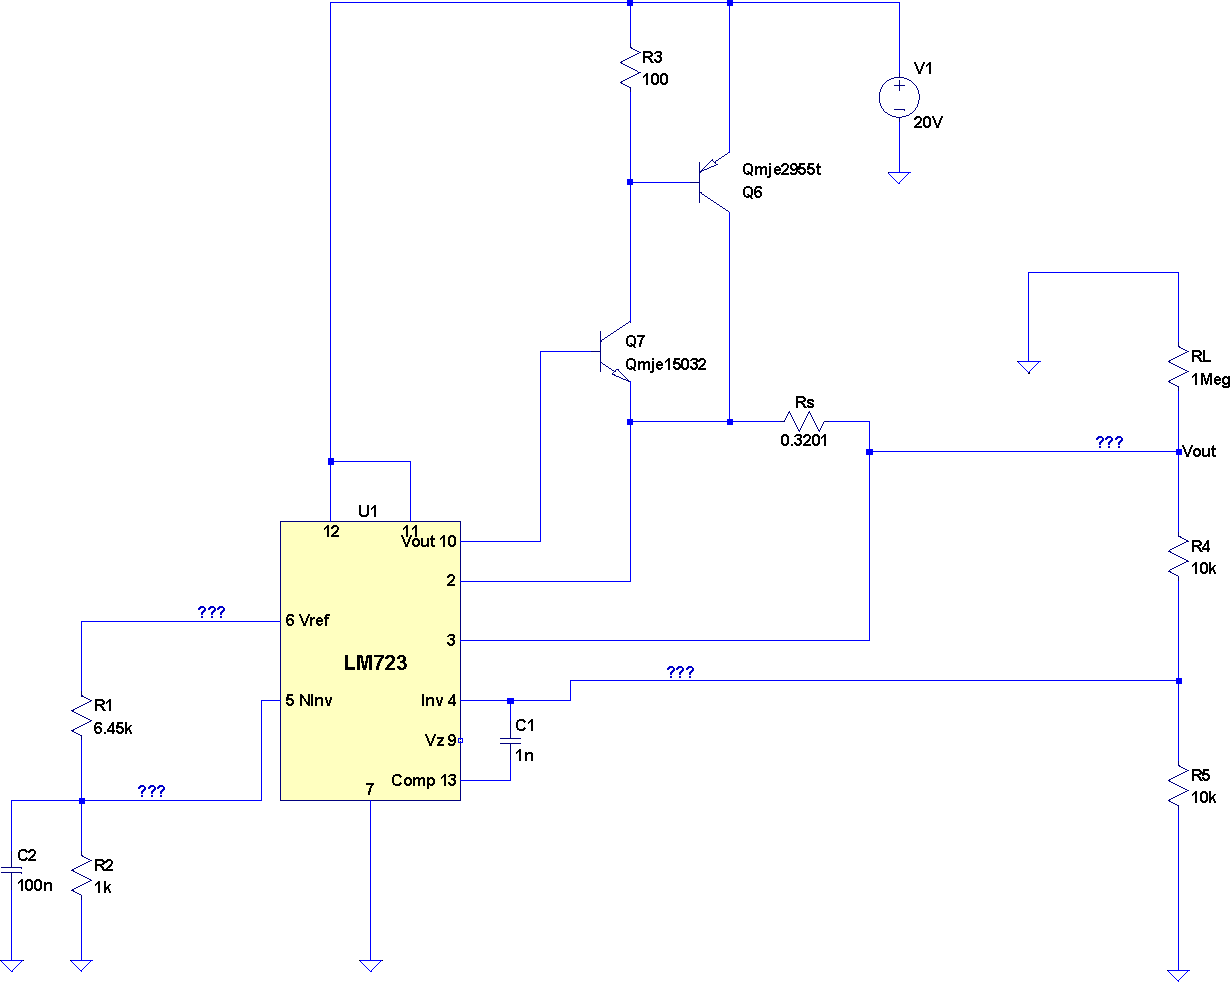
\includegraphics[width=1.2 \textwidth, angle=90]{./img/preguntas/p21.png}
\caption{\label{fig:fig_p21}\footnotesize{Rizado de entrada y salida.}}
\end{center}
\end{figure}

\clearpage

\subsubsection{Punto 6}


En la figura~\figref{fig:fig_p21_p6_output_voltage} se muestra el gráfico de la tensión de salida en modo de regulación de tensión en función de la resistencia del resistor $R_{9}$, el gráfico se obtuvo realizando una simulación paramétrica con $R_{L} = 1 \si[per-mode=symbol]{\mega\ohm}$, con el comando \textbf{SPICE} \textit{.step}, y luego se exportó el resultado y se graficó en \textbf{MATLAB}. En el gráfico se puede apreciar que, como se espera según lo calculado, el crecimiento es lineal con $R_{9}$, entre valores muy cercanos a los nominales de $1 \si[per-mode=symbol]{\volt}$ y $10 \si[per-mode=symbol]{\volt}$.




\vfill

\clearpage

\begin{figure}[H] %htb
\begin{center}
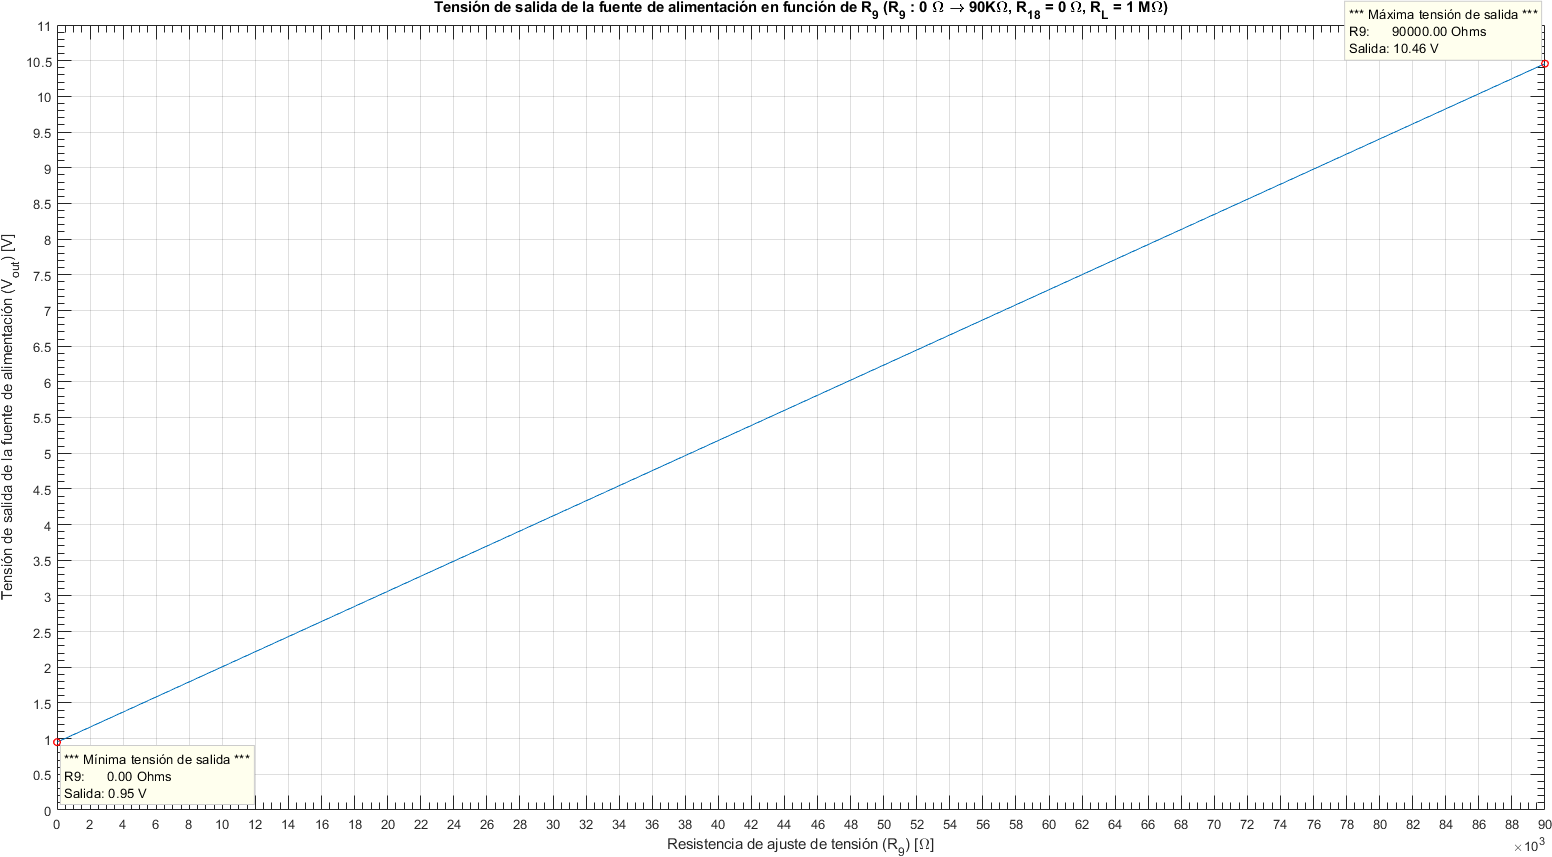
\includegraphics[width=1.2 \textwidth, angle=90]{./img/preguntas/p21_6.png}
\caption{\label{fig:fig_p21_p6_output_voltage}\footnotesize{Tensión de salida, $V_{o}$, en función de $R_{9}$, con esta variando entre $0 \si[per-mode=symbol]{\ohm}$ y $90 \si[per-mode=symbol]{\kilo\ohm}$.}}
\end{center}
\end{figure}



\clearpage


\subsubsection{Punto 13}


En la figura~\figref{fig:fig_p21_p13_output_impedance} se muestra el gráfico de la impedancia en el nodo de salida en modo de regulación de tensión, el gráfico se obtuvo simulando en \textbf{SPICE} con $R_{L} = 100 \si[per-mode=symbol]{\ohm}$, con una fuente de corriente de señal conectada en paralelo con la carga, $I_{p}$, realizando un barrido en alterna de $0.1 \si[per-mode=symbol]{\hertz}$ a $100 \si[per-mode=symbol]{\kilo\hertz}$, con el comando \textbf{SPICE} \textit{.ac}, y luego obteniendo el cociente $\frac{V\left(I_{p}\right)}{I_{p}}$, el resultado se exportó y se graficó en \textbf{MATLAB}, en escala semilogarítmica, su módulo y su fase, se destacó el resultado a bajas frecuencias que representa la resistencia de salida a frecuencia bajas/medias. El bajo valor obtenido para esta resistencia ($473 \si[per-mode=symbol]{\micro\ohm}$) implica que se trata de una buena fuente de tensión, que en el caso ideal tiene resistencia de salida de $0 \si[per-mode=symbol]{\ohm}$, esto se debe a la gran ganancia de lazo en modo de regulación de tensión. Otra cosa que se puede observar es que al aumentar la frecuencia la impedancia aumenta, al caer la ganancia de lazo, y se torna inductiva, al menos hasta que la fase supera los $90 \si[per-mode=symbol]{\degree}$, esto parece indicar un efecto de resistencia negativa, la fuente entregaría energía de alterna (esto necesita mas análisis).



\clearpage

\begin{figure}[H] %htb
\begin{center}
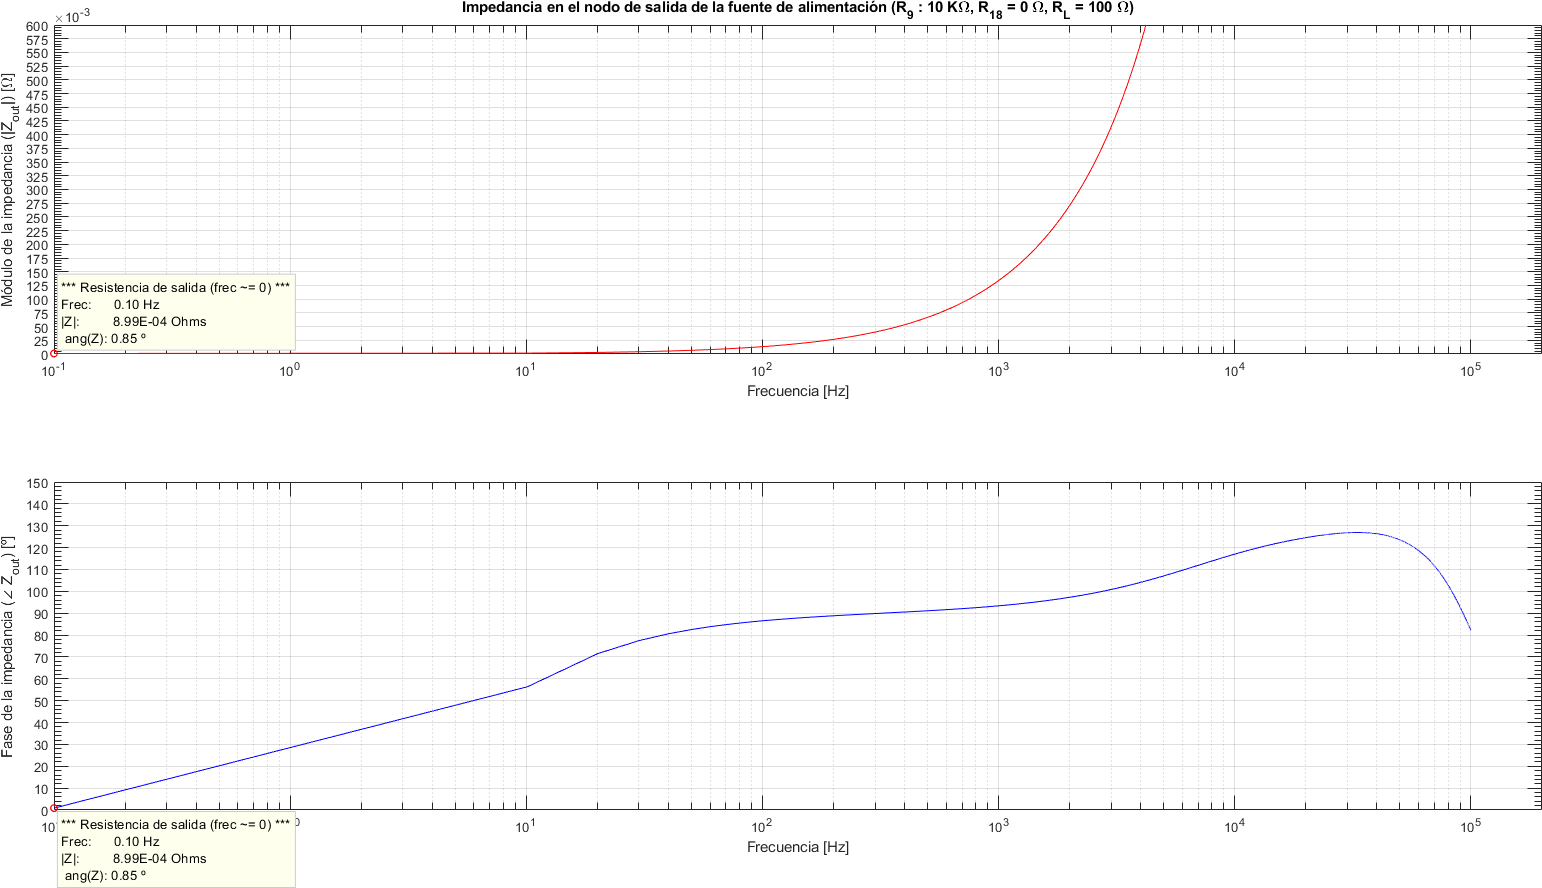
\includegraphics[width=1.2 \textwidth, angle=90]{./img/preguntas/p21_13.png}
\caption{\label{fig:fig_p21_p13_output_impedance}\footnotesize{Impedancia de salida, $Z_{o}$, en función de la frecuencia, con esta variando entre $0.1 \si[per-mode=symbol]{\hertz}$ y $100 \si[per-mode=symbol]{\kilo\hertz}$.}}
\end{center}
\end{figure}



\clearpage



\subsubsection{Punto 14}



En la figura~\figref{fig:fig_p21_p14_output_impedance} se muestra el gráfico de la impedancia en el nodo de salida en modo de regulación de corriente, el gráfico se obtuvo simulando en \textbf{SPICE} con la salida cortocircuitada a través de una fuente de tensión de señal, $V_{p}$, realizando un barrido en alterna de $0.1 \si[per-mode=symbol]{\hertz}$ a $100 \si[per-mode=symbol]{\kilo\hertz}$, con el comando \textbf{SPICE} \textit{.ac}, y luego obteniendo el cociente $\frac{V_{p}}{I\left({V_{p}}\right)}$, el resultado se exportó y se graficó en \textbf{MATLAB}, en escala semilogarítmica, su módulo y su fase, se destacó el resultado a bajas frecuencias que representa la resistencia de salida a frecuencia bajas/medias. El bajo valor obtenido para esta resistencia ($958 \si[per-mode=symbol]{\ohm}$) implica que no se trata de una buena fuente de corriente, que en el caso ideal tiene resistencia de salida $\infty$, esto se debe a la menor ganancia de lazo en modo regulación de corriente respecto al modo regulación tensión. Otra cosa que se puede observar es que al aumentar la frecuencia la impedancia disminuye, al caer la ganancia de lazo, y se torna capacitiva.



\clearpage

\begin{figure}[H] %htb
\begin{center}
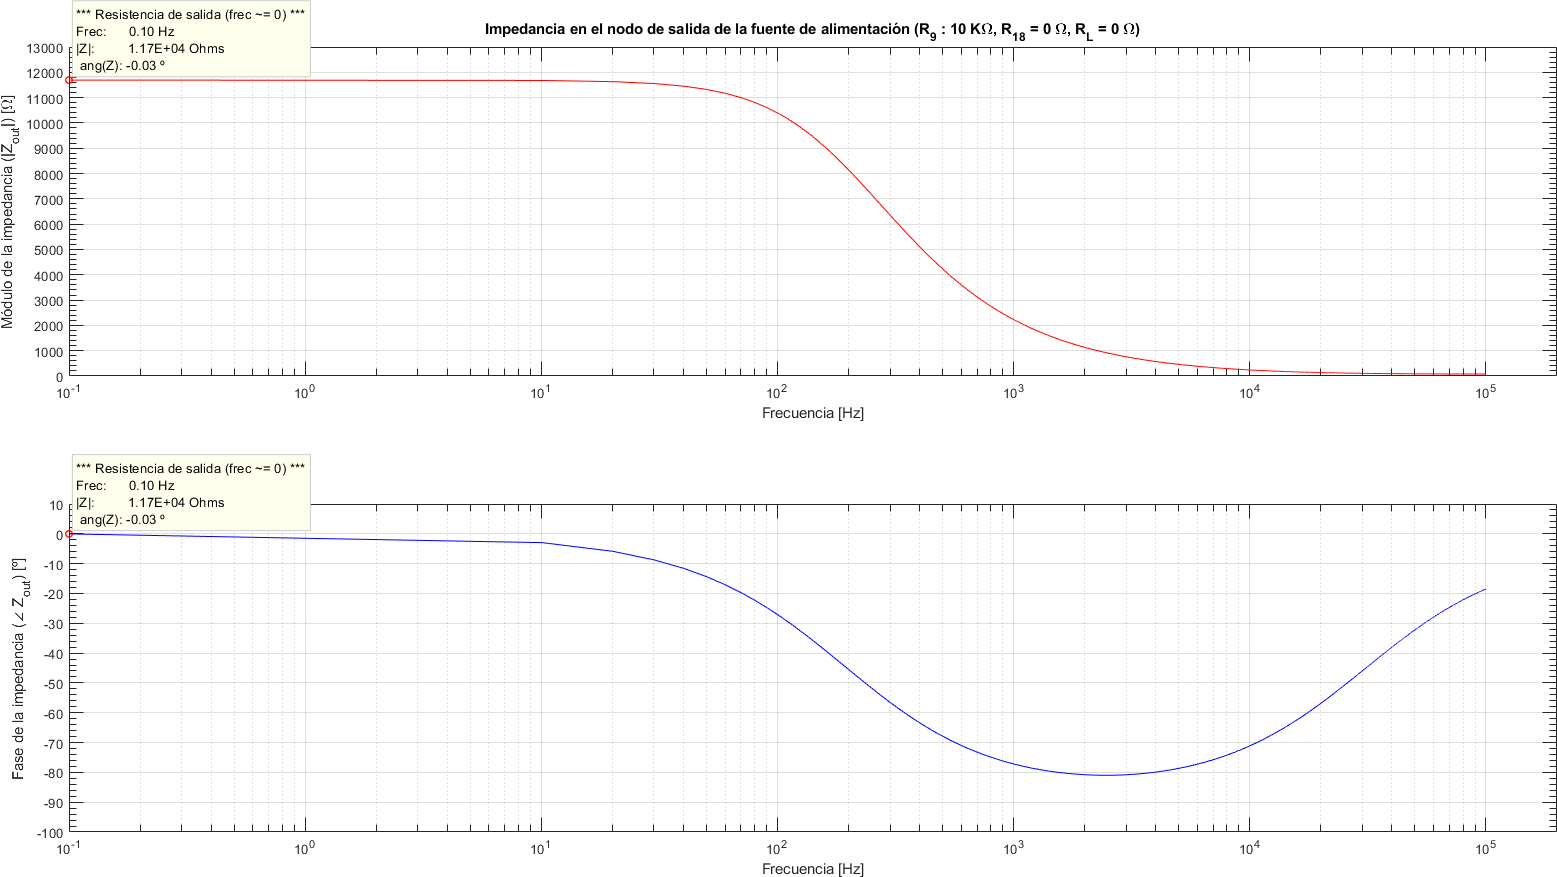
\includegraphics[width=1.2 \textwidth, angle=90]{./img/preguntas/p21_14.png}
\caption{\label{fig:fig_p21_p14_output_impedance}\footnotesize{Impedancia de salida, $Z_{o}$, en función de la frecuencia, con esta variando entre $0.1 \si[per-mode=symbol]{\hertz}$ y $100 \si[per-mode=symbol]{\kilo\hertz}$.}}
\end{center}
\end{figure}



\clearpage



\subsubsection{Punto 15}







En la figura~\figref{fig:fig_p21_p15_voltage_vs_current} se muestra la variación de la tensión de salida en función de la corriente de salida, se distinguen claramente y están marcadas, las regiones de regulación de tensión (la tensión nominal esperada es de $2 \si[per-mode=symbol]{\volt}$) y corriente (la corriente esperada es de $2 \si[per-mode=symbol]{\ampere}$).



\clearpage

\begin{figure}[H] %htb
\begin{center}
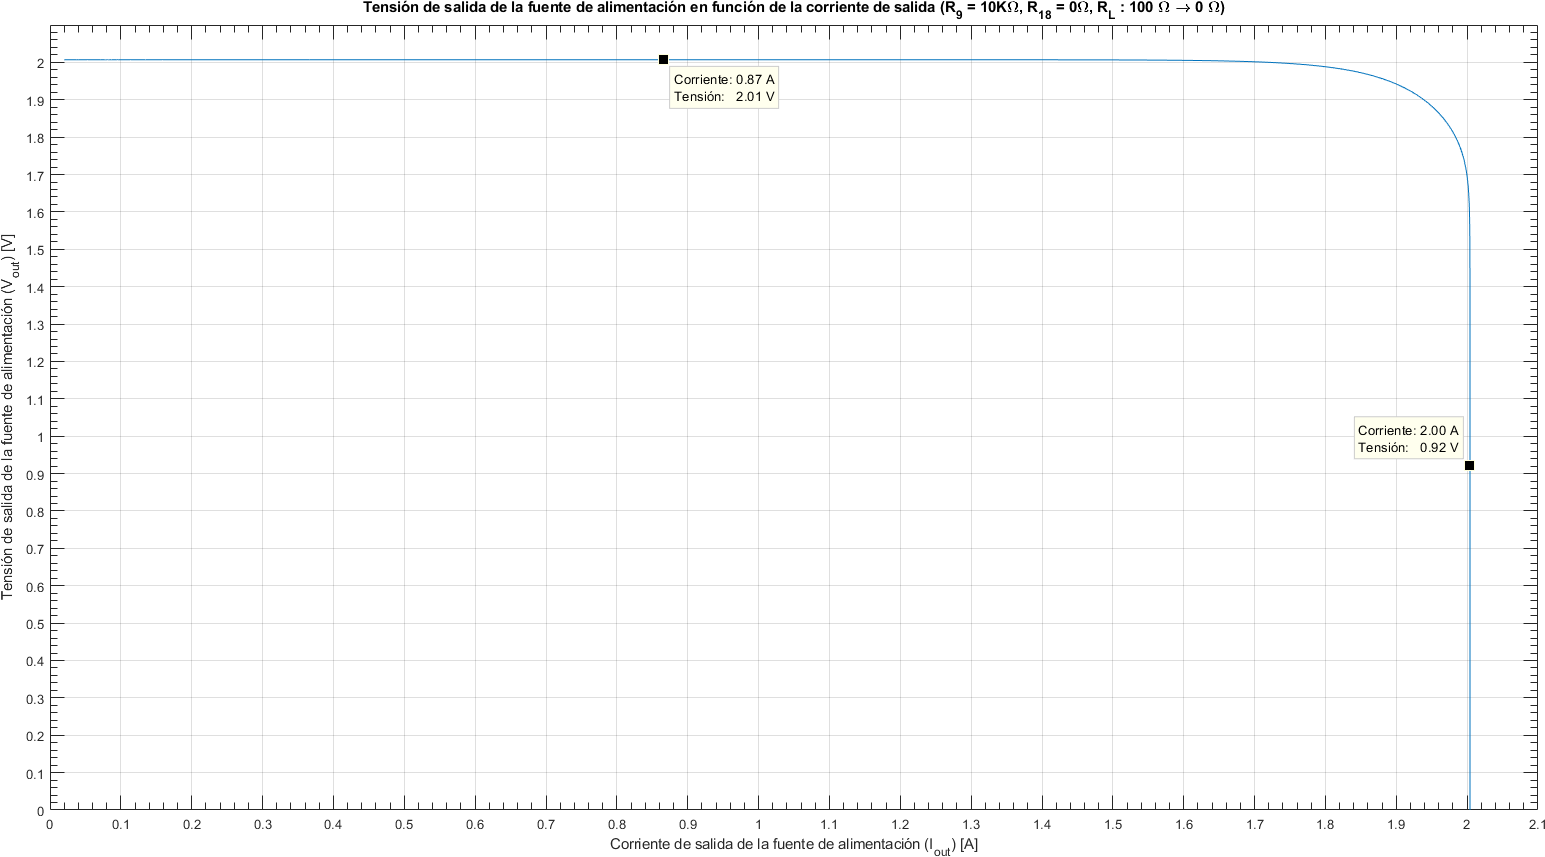
\includegraphics[width=1.2 \textwidth, angle=90]{./img/preguntas/p21_15.png}
\caption{\label{fig:fig_p21_p15_voltage_vs_current}\footnotesize{Tensión de salida en función de la corriente de salida para $R_{L}$ variando entre $100 \si[per-mode=symbol]{\ohm} y 0 \si[per-mode=symbol]{\ohm}$.}}
\end{center}
\end{figure}



\clearpage



\subsubsection{Punto 18}



Es de esperarse que la fuente tenga un valor mínimo de tensión de entrada, a partir del cual empieza a regular la salida, para valores menores de tensión que este valor mínimo, la salida será menor a la esperada, en principio, el regulador paralelo para regular a $10 \si[per-mode=symbol]{\volt}$, necesita una tensión de entrada mayor, pero también se deben polarizar correctamente los transistores, y como puede verse en la figura~\figref{fig:fig_p21_p18_vo_vs_vi}, el crecimiento de la salida es prácticamente lineal, manteniendo una diferencia de aproximadamente $2.2 \si[per-mode=symbol]{\volt}$ a la salida con respecto a la entrada, este valor sería el \quotemarks{drop-out} de esta fuente de alimentación. Tomando que la salida está regulando al 
llegar a aproximadamente al $1 \%$ de la tensión regulada esperada a la salida, $10 \si[per-mode=symbol]{\volt}$, el valor de tensión de entrada mínimo para salida regulada es de $12.38 \si[per-mode=symbol]{\volt}$. También puede observarse que para tensiones muy pequeñas a la entrada, hasta aproximadamente $1.8 \si[per-mode=symbol]{\volt}$, la tensión a la salida es prácticamente $0 \si[per-mode=symbol]{\volt}$, esto se explica por estar cortado el elemento de paso de la fuente de alimentación, el par compuesto.

\vfill

\clearpage

\begin{figure}[H] %htb
\begin{center}
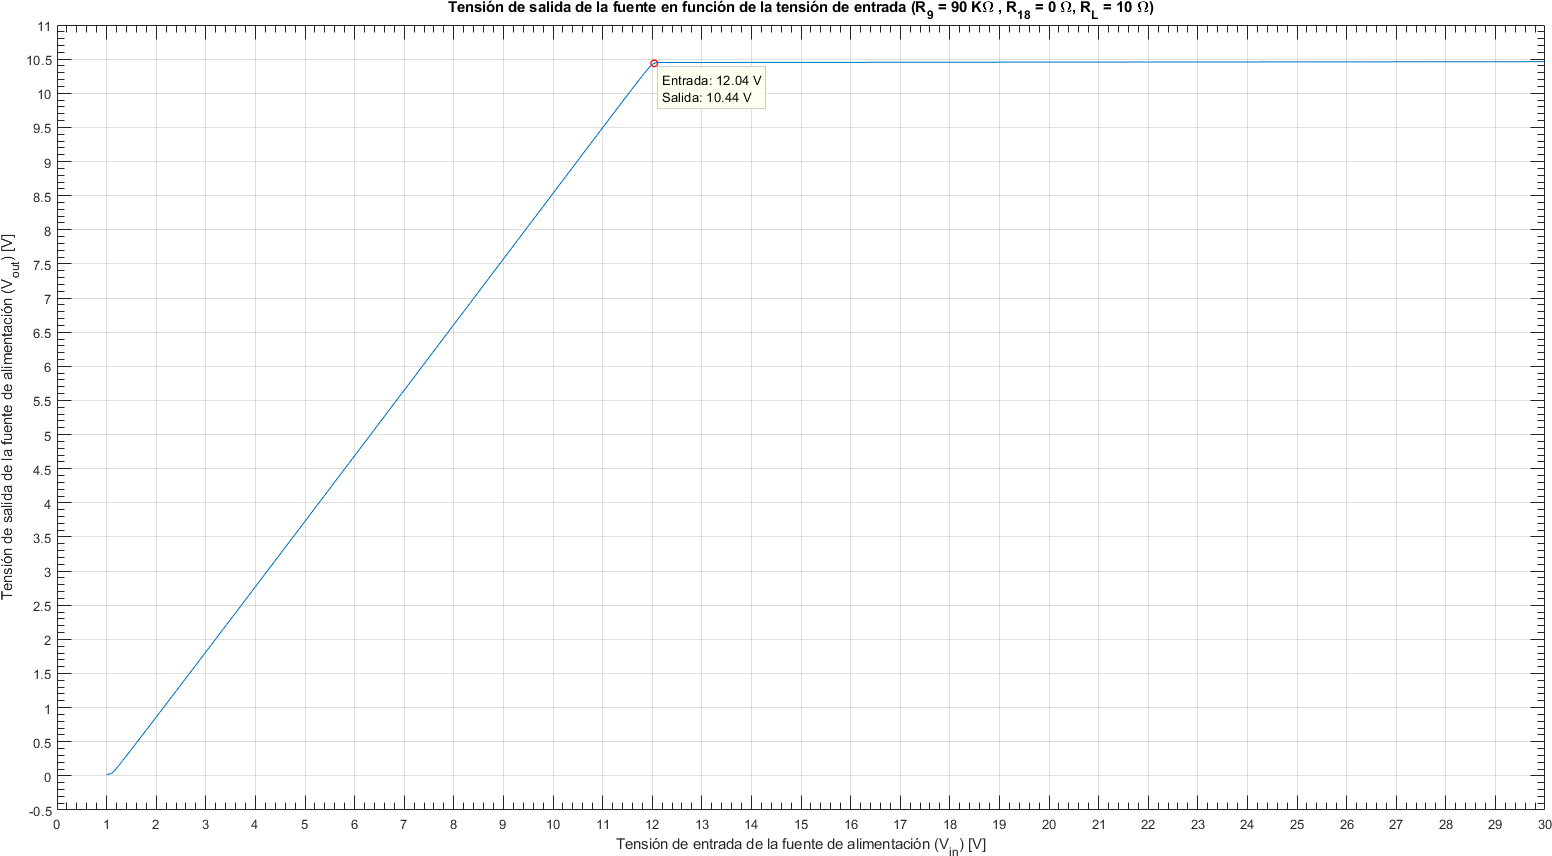
\includegraphics[width=1.2 \textwidth, angle=90]{./img/preguntas/p21_18.png}
\caption{\label{fig:fig_p21_p18_vo_vs_vi}\footnotesize{Tensión de salida vs tensión de entrada.}}
\end{center}
\end{figure}

\clearpage






